%\documentclass[10pt,a4paper]{article}
%\usepackage[latin1]{inputenc}
%\usepackage{amsmath}
%\usepackage{amsfonts}
%\usepackage{amssymb}
%\author{}
%\title{}
%\begin{document}




\providecommand{\abs}[1]{\left\lvert#1\right\rvert}
\tableofcontents
\listoffigures
\pagebreak
\section{Introduction}

The study of two-particle correlations at low relative momentum is commonly known as femtoscopy.  Femtoscopic analyses are capable of measuring spatio-temporal characteristics of heavy-ion collisions, with a particular emphasis made on estimating the homogeneity lengths (also called radii) of the particle-emitting source.  These analyses traditionally study pions \cite{Goldhaber:1960sf,Aamodt:2011mr} because of their ready availability and sensitivity to the spatial scale of the source.  However, measurements of heavier particles such as kaons \cite{Abelev:2012ms} and baryons \cite{Gos:2007cj} can serve to complement the pion results.  One motivation for studying an assortment of heavier particles is to test the hydrodynamic prediction that radial flow should cause the source radii to scale with the transverse mass $m_{\mathrm{T}}$ of the particles \cite{Csorgo:1995bi,Lisa:2005dd}.

Baryon--(anti)baryon correlation functions are also useful in the study of final state interactions (FSI).  Measurements of scattering lengths of pairs such as p$\Lambda$ and $\Lambda\Lambda$ are of interest for rescattering calculations, and, in the latter case, for understanding the properties of neutron stars \cite{SchaffnerBielich:2008kb,Wang:2010gr}.  Baryon-antibaryon correlations allow for the study of annihilation processes.  It has been argued that annihilation in the hadronic rescattering phase should be taken into account when determining particle yields \cite{Werner:2012xh,Karpenko:2012yf,Steinheimer:2012rd}.  This annihilation should result in an anticorrelation in baryon-antibaryon correlation functions.  Results from these femtoscopic analyses may be able to provide insight into the $p/\pi^+$ ratio measured in experiments at the LHC, which falls short of thermal model expectations \cite{Preghenella:2012eu}. 

In this note, we present two-$\Lambda$ momentum correlation functions measured in PbPb collisions at $\sqrt{s_{NN}}=2.76$ TeV by the ALICE Collaboration.  Results are shown for $\Lambda\Lambda$, $\bar{\Lambda}\bar{\Lambda}$ and $\Lambda\bar{\Lambda}$ pairs. The $\Lambda\bar{\Lambda}$ results are presented as a candidate for preliminary status. The motivation for $\Lambda$ baryon femtoscopy is to complement previous studies, as well as to probe the little-understood strong interactions of these baryons.


The primary effect seen in $\Lambda\bar{\Lambda}$ correlations should be strong final state interactions (FSI).  A suppression of the correlation function at low-$q_{\rm inv}$ is expected due to interactions in the baryon-antibaryon annihilation channel.  Suppressions of this sort have also been seen in $p \bar{p}$ interactions \cite{Gos:2007cj}, though the effects of this channel in charged particle studies can be somewhat obfuscated by Coulomb enhancement effects in the same $q_{\rm inv}$ region.  Also discussed in this note are the main influences on $\Lambda\Lambda$ correlations --- strong FSI and Fermi-Dirac statistics.  A long-term goal of this study is to measure characteristics of the interaction potential of the $\Lambda$ baryons.  More specifically, the scattering length $f_0$ and effective radius $d_0$ of the interaction can be extracted from two-$\Lambda$ correlations. It should also be noted that the H-dibaryon is thought to have two $\Lambda$s as one of its decay channels \cite{PhysRevLett.38.195}.  The study of $\Lambda$ momentum correlations at ALICE may some day provide measurements of this phenomenon, though endeavors in this direction are too preliminary to report upon at this time.

\section{Data analysis}
\subsection{Data selection}
\label{sec:DataSelection}
The analysis was performed on 31 July, 2013 using AliRoot v5-04-64-AN. The data were from PbPb collisions at $\sqrt{s_{NN}}=2.76$  TeV taken from the LHC11h (AOD115) pass 2 reconstruction. Runs were selected if they were listed with a pass 2 global quality of 1 ("Good run") in the Run Condition Table. Approximately 66 million combined central, semi-central and minimum bias events were analyzed. The following runs were used, which comprise both the positive (++) and negative magnetic (--) field orientations:

170593, 170572, 170388, 170387, 170315, 170313, 170312, 170311, 170309, 170308, 170306, 170270, 170269, 170268, 170230, 170228, 170207, 170204, 170203, 170193, 170163, 170159, 170155, 170091, 170089, 170088, 170085, 170084, 170083, 170081, 170040, 170027, 169965, 169923, 169859, 169858, 169855, 169846, 169838, 169837, 169835, 169591, 169590, 169588, 169587, 169586, 169557, 169555, 169554, 169553, 169550, 169515, 169512, 169506, 169504, 169498, 169475, 169420, 169419, 169418, 169417, 169415, 169411, 169238, 169167, 169160, 169156, 169148, 169145, 169144, 169138, 169099, 169094, 169091, 169045, 169044, 169040, 169035, 168992, 168988, 168826, 168777, 168514, 168512, 168511, 168467, 168464, 168460, 168458, 168362, 168361, 168342, 168341, 168325, 168322, 168311, 168310, 168115, 168108, 168107, 168105, 168076, 168069, 167988, 167987, 167985, 167920, 167915

Analysis was also performed on the LHC12a17a\_fix Monte Carlo HIJING run, which corresponds to the ++ field orientation events of the LHC11h anchors.  Approximately 650 thousand events were analyzed from runs

170593, 170572, 170388, 170387, 170315, 170313, 170312, 170311, 170309, 170308, 170306, 170270, 170269, 170268, 170230, 170228, 170207, 170204, 170203, 170193, 170163, 170159, 170155, 170091, 170089, 170088, 170085, 170084, 170083, 170081, 170040, 170027, 169965, 169923, 169859, 169858, 169855, 169uncorrected846, 169838, 169837, 169835

In all cases, the z-position of the primary vertex was required to be within 10 cm of the center of the ALICE detector for an event to be selected.  

\subsection{Detector use}
Both the data analysis as well as the MC analysis utilized information from several different detectors.  Event centrality was measured using the V0 detector with a timing cut from the Zero Degree Calorimeter.  The Inner Tracking System (ITS), Time Projection Chamber (TPC), Transition Radiation Detector (TRD), and Time of Flight detector together provided global tracking for the daughter particles.  Particle identification (PID) was performed using the TPC, as well as using the Time of Flight detector (TOF) when possible.

\subsection{$\Lambda$ reconstruction}
\label{sec:Recon}

During V0 reconstruction, a list of potential $\Lambda(\bar{\Lambda})$ candidates were extracted using the AliAODv0 Offline finder. The following cuts were applied for each V0's daughter tracks.

\begin{itemize}
\item The V0 was required to have no more than two daughters, and those daughters were required to have different charges.
\item The daughter tracks were required to have hits on at least 80 pad rows of the TPC.
\item The daughter protons (antiprotons) were required to have $p_{\rm T} > 0.5 (0.3)$ GeV/c, and the daughter pions required $p_{\rm T} \geq 0.16$ GeV/c.  All daughters were required to be in the range $|\eta| < 0.8$.
\item The TPC was used for PID purposes.  For proton and pion daughter candidates, the PID resolution task was used to obtain NSigma, which was required to be less than 3.
\item Daughter tracks were required to have a TOF PID NSigma value less than 4 if the TOF signal was available.
\item The two daughters are required to have a DCA $< 0.4$ cm to each other.
\item The daughters were each required to have a DCA to the primary vertex $> 0.1$ cm.
\end{itemize}

Each V0 is then subjected to the following cuts:
\begin{itemize}
\item The V0 is required to have $|\eta| < 0.8$.
\item The cosine of the pointing angle must be greater than 0.998.
\item The DCA of the V0 to the primary vertex must be less than 1 cm.
\item For a $\Lambda$, one daughter must be identified as a proton and the other as a $\pi^-$.  For a $\bar{\Lambda}$, one daughter must be identified as an antiproton and the other as a $\pi^+$.
\item For both $\Lambda$ and $\bar{\Lambda}$, the reconstructed invariant mass was required to fall within $\abs{m_\mathrm{inv}-m_\mathrm{PDG}} < 5.68$ MeV.
\end{itemize}

The optimal cut values were determined by comparing cut distributions of reconstructed $\Lambda$ in Monte Carlo HIJING events (including simulated detector effects). $\Lambda$ were reconstructed and their corresponding AliAODMCParticle objects were consulted in order to classify the $\Lambda$ into different categories: Real, primary $\Lambda$; secondary $\Lambda$ coming from decays of $\Sigma$ (or $\Sigma$ excited states), $\Xi$, and $\Omega$; secondary $\Lambda$ coming from other sources; fake $\Lambda$; and $K^0_\mathrm{s}$ that have been misidentified as $\Lambda$.  For each cut parameter (e.g. cosine of pointing angle), a plot was made showing the distributions of V0 candidates of the various types.  These plots contain only the parameter distributions of candidates that pass all the other cuts.  Figures \ref{fig:CosP,fig:DcaV0,...} show these distributions for the different particle types.  

\begin{figure}
%distribution figures
\end{figure}

For the construction of Figures \ref{fig:CosP,fig:DcaV0,...}, each $\Lambda$ type was preselected using AliAODMCParticle information, and only V0 candidates of that type were reconstructed in that analysis run. This was done for ease of histogramming the distributions.  Roughly equal numbers events were analyzed for each run type, with the exception of the analysis of the primary $\Lambda$.  That analysis run utilized only about half the data set.  Therefore, the primary $\Lambda$ distributions in Figures \ref{fig:CosP,fig:DcaV0,...} have been scaled by a factor of 2 to compensate.

In these figures, both the shape and magnitude of each distribution is relevant for determining the cuts. For each cut type, a cut value was selected such that a looser cut would differentially accept more fake or secondary $\Lambda$ than primary $\Lambda$. Ideally, these cuts would be selected to reduce the inclusion of all types of secondary $\Lambda$.  However, it can be seen from the distributions that $\Lambda$ that come from $\Sigma$ decay display virtually the same cut parameter distribution shapes as primary $\Lambda$.  Only the magnitude of the $\Sigma$ curves differ from the primary $\Lambda$ curves.  This is due to the short decay length of the $\Sigma$ decay: ...dl... for $\Sigma$ ...smaller mass..., and ...dl... for $\Sigma$1385. As a result, secondary $\Lambda$ from $\Sigma$ look identical to primary $\Lambda$, and they cannot be selectively removed from the analysis.

The systematic errors associated with these cut choices are discussed in Section \ref{sec:sec:SystematicsReconstruction}. Further discussion of the reconstruction efficiency of the different $\Lambda$ types can be found in Section \ref{sec:ReconstructionEff}.

The reconstructed invariant mass spectra for $\Lambda$ can be seen in Figure \ref{fig:LambdaInvMass}. An approximation of the signal purity was estimated using a ratio of real and background (falsely reconstructed) counts.  The background was estimated using a fourth order polynomial.  The number of real $\Lambda$ was then estimated by counting the bin content and subtracting the background. The signal quality was found to be $real/(real + background) \approx 0.82$ ********Update this **********.

%Figure \ref{fig:MassTightCut} shows the invariant mass spectra when tighter cuts are enforced.  The cuts increase the minimum DCA of the daughters to the primary vertex to 1 cm, reduced the max DCA of the V0 to the primary vertex to 0.8 cm, and set a minimum decay length of 2 cm.  These cuts ensure a better purity by eliminating much of the contamination of the reconstruction by primary particles.  However, there is also a significant drop ({\raise.17ex\hbox{$\scriptstyle\mathtt{\sim}$}} threefold) in the number of reconstructed $\Lambda$, as well as the number of $\Lambda$ pairs.  While these cuts afford a higher purity, the extracted correlation function was found to be less significant due to the decreased statistics.  Therefore, the looser cuts defined in Section \ref{sec:Recon} are preferred.  Further details are discussed in Section \ref{sec:Systematics}.

\subsection{Shared daughter cut}

Occasionally two or more V0s are reconstructed that both claim the same daughter track.  However, a given track can only be the daughter of, at most, one V0.  Therefore, if several reconstructed V0s all lay claim to the same daughter, at most only one of them can be a true V0.  It was decided to employ a cut that would compare characteristics of the different V0s to determine which of them was most likely to be the true parent particle.  After the best V0 was found, the competing V0s were removed from the list of V0 particles and not used during same- or mixed-event pair construction.

A study was done using MC event truths to determine which cut would be most successful at removing fraudulent V0s.  The following characteristics were examined:

\begin{itemize}
\item Closeness of invariant mass to the PDG mass value.
\item DCA of the daughter particles to each other.
\item Cosine of the pointing angle.
\item DCA of the V0 to the primary vertex.
\end{itemize}

Based on the MC truth study, the ... cut was found to successfully keep true V0s and remove fake V0s ...\% of the time.  

On average there were two competing particles per every ... events in the MC study.  When applied to analysis of the LHC11h data, the rate was two per ....

In order to keep spurious correlated signals from entering the correlation functions, a cut on daughter particles was implemented.  After all the V0s in an event were reconstructed, the V0s were checked to see if they shared any daughters.  Those V0s that shared a daughter were compared via several characteristics:

As this shared-daughter cut process was done sequentially through the ... an iterative process was developed to ensure... 

(example: V0s "A" and "B" both share a daughter, and V0s "A" and "C" share a different daughter.  "A" has a better DCA than "B", so "B" is removed.  Then "C" is found to have a better DCA than "A", so "A" is removed.  Finally, "B" is returned because it no longer competes for a daughter).

This cut helps remove a splitting-like effect (see sec \ref{sec:PairWiseCuts} for more on splitting), wherein one true V0 has each of its daughters claimed by two separate fake V0s.  By the nature of the reconstruction cuts, all three of the V0s will be close in momentum space.  Therefore a pair constructed from the two fake V0s will contaminate the low relative-momentum region of the correlation function.  


\subsection{Correlation function construction and pair cuts}
\label{sec:CFconstruct}

This analysis studies two-particle correlations as a function of the one dimensional relative momentum $k^*=\frac{1}{2}q_{\mathrm{inv}}=\frac{1}{2}\abs{P(m^2_1-m^2_2)/P^2 - q}$, where $P$ and $q$ are the four-vector momentum sum and difference, respectively, and $m_1$ and $m_2$ are the masses of the two particles.  The correlation function is constructed as $C(k^*) = A(k^*)/B(k^*)$, where $A(k^*)$ is the two-particle distribution of the given event and $B(k^*)$ is the distribution of a reference event.  In practice, the signal event histogram $A(k^*)$ is constructed by binning the $k^*$ value of each pair of particles in a single event, and repeating this for each event.  The reference (or background) histogram is constructed by binning $k^*$ for pairs of particles taken from different events.  Care is taken to ensure that pairs are mixed from events with similar centralities (bin width of 5\%) and primary vertex z-position (2 cm bin width).  There are five mixed events for each real event.  When constructing pairs of V0s from the same event, the V0s are not allowed to share a daughter with the same track id. 

\subsection{Pair-wise cuts}
\label{sec:PairWiseCuts}

Femtoscopic studies look at the relative momentum of particles, and often the most interesting physics lies at very low relative momentum (around 0.1 GeV/c and lower).  As a result, two-track reconstruction effects such as track splitting and track merging, both of which occur for tracks with similar momenta and trajectories, can have a large effect on the final results.  Track splitting means that the track left by a single charged particle is reconstructed as two separate tracks. Track merging is when the tracks of two separate particles are reconstructed as a single track.  For V0s, splitting/merging occurs on the level of the daughter tracks, and it affects the reconstruction of the parent V0s.

In this analysis, two-track reconstruction effects are combatted via a cut on the average separation of daughter tracks from different lambdas.  The average separation distance of two daughter tracks are computed at nine different radii of the TPC.  The tracks are propagated iteratively using their local coordinates and the PropagateTo function, and their global positions are determined at 85, 105, 125, 145, 165, 185, 205, 225, and 245 cm.  Initial iteration is performed in 1 cm steps, though a secondary propagation is done in 0.1 cm steps for better precision.  Same- and mixed-event pairs are binned according to this separation distance.  To obtain an estimate of the merging/splitting effects both distributions are then scaled by the number of pairs at high average separation distance (10+ cm), and a correlation function (same event pairs/ mixed event pairs) is created. 

To ensure that average separation distributions of mixed-event pairs are comparable to the same-event distributions, it is necessary to perform a shifting of the primary vertex for mixed events.  Doing so allows the track separations to be calculated as though both events had the same primary vertex.  Without this correction, the mixed-event distributions are biased by differences in the primary vertex location.  One could imagine an extreme example of this if one used a 20 cm wide z-vertex bin.  In that case, tracks from different events could be shifted relative to each other by as much as 20 cm.  For this analysis with 2 cm z-vertex binning, and the uncorrected average separation correlation is shown in Figure \ref{ref:TwoTrackPerf} (left panel).  In contrast, the right panel of Figure \ref{fig:TwoTrackPerf} shows the primary-vertex corrected correlation.  To get a clear account of the difference between the two, we can look at Figure \ref{fig:TwoTrackRatio}, which shows the ratio of the corrected to uncorrected correlations.  The ratio is above unity from between 0 and 4cm.  We can interpret this to mean that the vertex-corrected distribution has more splitting and less merging than we would expect from the uncorrected plot.

Looking at Figure \ref{ref:TwoTrackPerf}, one can see that splitting effects are relevant out to about 1 cm, as evidenced by a relative abundance of same-event pairs.  Merging is visible out to about 3 cm, as evidenced by a dearth of same-event pairs in that range.  To address these effects, both same- and mixed-event V0 pairs are cut if they have a like-sign daughter pair with average separation less than 3 cm.  

However, one must be somewhat cautious here, since there are physics reasons to expect that $\Lambda\Lambda$ and $\Lambda\bar{\Lambda}$ should be suppressed at low relative momentum.  Some of that natural, physics-driven suppression may show up as a suppression in the average separation plots of the daughter tracks.  

One alternative/complement to using an average separation cut would be to enforce a relative decay length cut, where V0s are not paired with each other if their difference between their lab frame decay length values is less than some cut value (e.g. a few cm).  One advantage of this cut is that the decay lengths of the various particles should be independent of physics effects - i.e. independent of any quantum interference or final state interaction that might occur between the particles.  Meanwhile, the decay length cut may minimize daughter splitting effects, as well as some merging of low- and mid-$p_{\mathrm{T}}$ daughters.  High-$p_{\mathrm{T}}$ daughters may still be affected by merging, since higher-$p_{\mathrm{T}}$ particles have straighter trajectories in the TPC.  An analysis of relative decay length has not been performed yet, but it may prove a useful to combat splitting/merging effects.


%  In contrast, the average separation cut likely cuts out not only splitting/merging, but also some pairs with legitimate physics affects, since particles with low average separation are also close in relative momentum.  In the V0 case, neutral particles whose daughters are nearly collinear (i.e. small average separation) are themselves.


%\begin{figure}[hbtp]
\begin{figure}[h]
\begin{minipage}{18pc}
%\includegraphics[scale=0.6]{Figures/2013-09-15-TwoTrackPerfUncorrected.pdf}
\includegraphics[width=18pc]{Figures/2013-09-15-TwoTrackPerfUncorrected.pdf}
\end{minipage}\hspace{2pc}
\begin{minipage}{18pc}
\includegraphics[width=18pc]{Figures/2013-09-15-TwoTrackPerfCorrected.pdf}
\end{minipage} 
\caption[Two-track reconstruction effects]{\label{ref:TwoTrackPerf}Correlation function versus average separation distance in the TPC for proton daughters.  Constructed using same-event pairs over uncorrected mixed-event pairs.  Both splitting (enhancement) and merging (suppression) effects are visible. The left panel shows the distribution with uncorrected mixed-event pairs, while the right panel shows the distributions with proper primary-vertex correction treatment.}
\end{figure}

\begin{figure}[hbtp]
\includegraphics[width=18pc]{Figures/2013-09-15-TwoTrackRatio.pdf}
\caption[Ratio of corrected/uncorrected average-separation distributions]{Ratio of vertex-corrected average separation plot to uncorrected average separation plot.  The enhancement above unity at low average-separation suggests that the uncorrected distribution underestimates the amount of splitting and overestimates the amount of merging.  The differences between the plots seems to disappear (i.e. ratio goes to unity at $\approx$ 3 cm.}
\label{fig:TwoTrackRatio}
\end{figure}

\section{Correlation function results}
\subsection{Correlation functions}
\label{sec:RawCorrelationFunctions}

%..... Discussion of correlation function data results and systematic uncertainties.  ......

%********Outdated****** some of this may be salvageable

Figure \ref{fig:CFMixCentralities} shows $\Lambda\bar{\Lambda}$ correlation functions versus $q_{\rm inv}$ for three different centralities ranges.  The correlations are normalized to unity in the $ 0.3 < q_{\rm_{inv}} < 0.5$ GeV/c range.  Each correlation shows clear suppression in the low-$q_{\rm_{inv}}$ region, which is considered an effect of the baryon-antibaryon annihilation channel.  The strength of the correlation effect increases with more peripheral events, an indication that the emitting source size is shrinking for those events.

Figure \ref{fig:CF} shows correlation functions constructed in the 0-10\% centrality range for $\Lambda\Lambda$ and $\bar{\Lambda}\bar{\Lambda}$ pairs.  Both correlation functions exhibit an enhancement in the low-$q_{\rm inv}$ range of 0.04 - 0.2 GeV/c.  This may be due to attractive final state interactions.  The effects of FSI and quantum statistics are expected to be seen in roughly the same $q_{\rm inv}$ range, and it is unclear at this time to what extent their effects should be competing. The enhancement of the $\bar{\Lambda}\bar{\Lambda}$ correlation function does fall off in the lowest bins, though the statistical uncertainties are such that no significant statement about the effects of quantum statistics can be made at this time.



\subsection{Systematic errors from reconstruction cuts}
label{sec:SystematicsReconstruction}

Discussion of systematic errors associated with V0 reconstruction cuts will go here.

\subsection{Systematic errors from pair-wise cuts}
label{sec:SystematicsReconstruction}

Discussion of systematic errors associated with pair-wise cuts will go here.

%********Outdated****** some of this may be salvageable

This analysis is in a preliminary phase where fit parameters such as source radii and correlation strength are unavailable.  Therefore a discussion of systematic effects is at this time limited to showing how different sets of cuts change the qualitative aspects of the correlation function plot.  The effects of two such cuts are discussed here.  An attempt is made to quantify the systematic uncertainty between these different cuts for the $\Lambda\bar{\Lambda}$ correlation function.

Two-track reconstruction effects were discussed in Section \ref{sec:PairWiseCuts}. Figure \ref{fig:CFNoMergeMix} shows the three centralities of $\Lambda\bar{\Lambda}$ correlation functions measured without the average separation cut in place.  Figure \ref{fig:CFNoMerge} shows the equivalent plot for the $\Lambda\Lambda$ and $\bar{\Lambda}\bar{\Lambda}$ correlations. Subtle differences are visible in the $q_{\rm inv} < 0.2$ GeV/c range, with the most drastic changes lying in the lowest bins where the statistics are the weakest.  Except for the lowest bin, the changes all fall within error bars of the points in Figures \ref{fig:CFMixCentralities} and \ref{fig:CF}.  Nonetheless, it is clear that including the two-track cuts  shifts the low-$q_{\rm inv}$ bins down by a noticeable amount, a sign that splitting effects are being removed.  This consistent downward shift indicates that two-track effects are a significant source of systematic error in this study.

As mentioned in Section \ref{sec:Recon}, two sets of reconstruction cuts (loose and tight) have been studied in detail.  Figure \ref{fig:CFMixCentralities} was created using loose reconstruction cuts.  For comparison, Figure \ref{fig:CFTightCutsMix} shows the same correlations with tighter reconstruction cuts employed.  Figure \ref{fig:CFTightCuts} shows a similar plot for the $\Lambda\Lambda$ and $\bar{\Lambda}\bar{\Lambda}$ correlations.  It is apparent that the statistics are much worse under the tigher cuts, though qualitative similarities to the other plots remain, e.g.\ the centrality dependence of the $\Lambda\bar{\Lambda}$ annihilation and the enhancement of the $\Lambda\Lambda$ and $\bar{\Lambda}\bar{\Lambda}$ at low-$q_{\rm inv}$.

A conservative estimate of the systematic errors for the $\Lambda\bar{\Lambda}$ correlation function and are shown in Figure \ref{fig:CFMixSystematics}.  The systematic errors were computed by taking the absolute value of the difference between Figure \ref{fig:CFMixCentralities} and Figure \ref{fig:CFTightCutsMix} for each $q_{\rm inv}$ bin.  The results were then fit with a 5th order polynomial.  The value of the polynomial was determined at the center of each $q_{\rm inv}$ bin.  This value was halved and then applied as a symmetric systematic error for that particular $q_{\rm inv}$ bin.  The data points and statistical errors are those from Figure \ref{fig:CFMixCentralities}.





\section{1D analytic model}
%\subsection{Analytical model}
With the assumption of a spherically gaussian source of width $R$, the 1D femtoscopic correlation functions can be calculated analytically \cite{lednicky82} using 

\begin{equation}
C(k^*)= 1 + C_1(k^*)+C_2(k^*)
\end{equation}
$C_1$ describes plane-wave quantum interference:
\begin{equation}
C_1(k^*) = \alpha e^{-4k^{*2}R^2}
\end{equation}
where $\alpha = (-1)^{2j}/(2j+1)$ for identical particles with spins $j$, and $\alpha = 0$ for non-identical particles.  $C_2$ describes the s-wave strong final state interaction of the particles:
\begin{equation}
\label{eq:Lednicky}
C_2(k^*)= 1+ (1+\alpha)\left[\frac{1}{2}\abs{\frac{f(k^*)}{R}}^2(1-\frac{d_0}{2\sqrt{\pi}R})+\frac{2\Re f(k^*)}{\sqrt{\pi}R}F_1(2k^*R)-\frac{\Im f(k^*)}{R}F_2(2k^*R)\right]
%C_2(k^*)= 1+ \displaystyle\sum\limits_{S}\rho_S\left[\frac{1}{2}\abs{\frac{f^S(k^*)}{R}}^2(1-\frac{d_0^S}{2\sqrt{\pi}R})+\frac{2\Re f^S(k^*)}{\sqrt{\pi}R}F_1(2k^*R)-\frac{\Im f^S(k^*)}{R}F_2(2k^*R)\right]
\end{equation}
where $F_1(z) = \int_0^z \! \mathrm{d}x \, e^{x^2-z^2}/z$,  $F_2(z) = (1-e^{-z^2})/z$, and $R$ is the source size. The $(1+\alpha)$ pre-factor accounts for the relevant (non/anti-)symmetrizaton effects.  $f(k^*)=(1/f_0+\frac{1}{2}d_0k^*-ik^*)^{-1}$ is the s-wave scattering amplitude, written using the effective range approximation.  The scattering amplitude is dependent upon the effective range of interaction $d_0$, as well as the complex scattering length $f_0$.  The real part of the scattering amplitude can contribute either a positive or a negative correlation, but either way the effect is relatively narrow in $k^*$ (on the order of about one hundred MeV/$c$).  The imaginary part of the scattering amplitude accounts for inelastic processes of baryon-antibaryon annihilation.  Introducing a non-zero imaginary part to the scattering length produces a wide (hundreds of MeV/$c$) negative correlation.  For charged particles, an additional factor \cite{Aamodt:2011kd} is necessary to account for the Coulomb interaction.

Techinically, the scattering length and effective range are spin dependent.  It should be noted that in the case of identical fermions, "the contributions of s-wave interaction of identical nucleons to the correlation function goes to zero [for summary spin state S = 1] (identical nucleons with parallel spins cannot be in the s-wave state)" \cite{lednicky82}.  As a result, only the spin singlet (i.e. antisymmetric spinor, symmetric spatial wave function) scattering parameters are measured for identical fermions.  Such is the case for the $\Lambda\Lambda$ and $\bar{\Lambda}\bar{\Lambda}$ correlation measurements.  However, for non-identical particles such as $\Lambda\bar{\Lambda}$, the factor $(1+\alpha)$ could be replaced with a weighted sum of $C_2$ calculated using separate spin-dependent scattering parameters.  That calculation would use $\rho_S$, the fraction of pairs in each total spin state S, as the weight.  For statistical reasons, this analysis will eschew spin-dependent measurements of the $\Lambda\bar{\Lambda}$ scattering parameters, and instead attempt to fit for a spin-averaged value.


\subsection{Observables}
\label{sec:Observables}
For pion, kaon, and proton femtoscopic analyses, the scattering lengths and effective radius of interaction are well specified by years of scattering data, and they can be fixed to the known values.  In the case of lambda-(anti-)lambda femtoscopy, the interaction is heretofore largely unstudied.  For this analysis, the scattering lengths and effective radius are left as free parameters.  Another free parameter is the $\lambda$ parameter, which is roughly a measure of the pair purity.  For example, $\lambda_{\Lambda\Lambda}$ would correspond to the ratio of number of true primary $\Lambda\Lambda$ pairs to the total number of pairs in the correlation function. The remaining fraction is comprised of all the other combinations of pair types, such as pairs where one $\Lambda$ is real and primary and the other is fake, or pairs between primary and secondary lambdas.  The latter case will be described further in Section \ref{sec:Residual}.  The last fit parameter is $R_{\rm inv}$, which characterizes the one dimensional size of the emitting source.  


\subsection{Residual correlations}
\label{sec:Residual}

Attempts at fitting correlation functions should try to account for residual correlations between the particle being studied and other particles that might decay into the studied particle.  Various particles can decay into $\Lambda$ baryons, such as $\Sigma^{\rm 0}$, $\Xi^{\rm 0}$, and $\Omega^{\rm -}$.  The decay momentum between these particles and their daughter $\Lambda$ is small, such that daughter and parent carry very similar momenta.  As a result, relative-momentum correlation functions between primary particles and secondary particles such as $\Lambda$ should be sensitive to the interactions between the primary particles and the parent particles.  For example, the correlation between primary $\Lambda$ and primary $\Sigma^{\rm 0}$ should be visible, though somewhat smeared out, in the correlation between primary $\Lambda$ and secondary $\Lambda$.  Furthermore, these secondary $\Lambda$ are often difficult to distinguish from primary $\Lambda$.  Therefore, measurements of two-$\Lambda$ correlation functions will contain a mixture of primary correlations and feeddown correlations, and an attempt to parametrize the correlation functions should take this into account.  

One example of this type of parametrization can be seen in the recent proton femtoscopy results from ALICE Pb--Pb collisions \cite{Szymanski:2012AN}.  In that study, initial attempts to fit a purely primary proton-proton correlation function failed to reproduce the shape of the data.  However, when further parametrization was introduced to take into account proton-proton correlations where one proton was primary and one came from a $\Lambda$ decay, the fit was remarkably successful.

We attempt to quantify the residual contamination in this analysis by simultaneously fitting the data for both the primary correlation function and the residual correlations.  For example, $\Lambda\Lambda$ correlations with $\mathrm{\Lambda\Sigma^0}$ feeddown would be fit using 

\begin{equation}
\label{eq:Residual}
C_{\mathrm{meas}}(k^*_{\Lambda\Lambda})= 1 + \lambda_{\Lambda\Lambda}[C_{\Lambda\Lambda}(k^*_{\Lambda\Lambda})-1]+\lambda_{\Lambda\Sigma}[C_{\Lambda\Sigma}(k^*_{\Lambda\Lambda})-1],
\end{equation}
where $$C_{\Lambda\Sigma}(k^*_{\Lambda\Lambda}) \equiv \displaystyle\sum\limits_{k^*_{\Lambda\Sigma}}C_{\Lambda\Sigma}(k^*_{\Lambda\Sigma})T(k^*_{\Lambda\Sigma},k^*_{\Lambda\Lambda}),$$ $C_{\Lambda\Sigma}(k^*_{\Lambda\Sigma})$ is the $\Lambda\Sigma$ correlation function calculated from Eq.~(\ref{eq:Lednicky}), and $T$ is a THERMINATOR \cite{Chojnacki:2011hb} transform matrix, which generates pairs of particles and determines kinematically how the $k^*$ of the pair transforms when one of the particles decays.  Figure \ref{fig:TherminatorLS} shows the transform matrix for $\Lambda\Sigma \rightarrow \Lambda\Lambda$.  Further residual correlations (e.g. from $\Sigma\Sigma \rightarrow \Lambda\Lambda$) can be included via additional terms in Equation \ref{eq:Residual}.  Efforts are underway to understand which residual correlations must be included and which can be safely neglected.  Section \ref{sec:LambdaParams} will discuss the current status of this analysis.

\section{Fitting results and systematics}
\label{sec:FittingSystematics}

Proper fitting techniques for this analysis are still a work in progress.  In particular, efforts are being made to evaluate the extent to which residual correlations permeate the measured correlation functions.  In this analysis, the importance of residual correlations can be characterized by two sets of parameters.  The scattering lengths $f_0$ of the residual pair describe the strength of the residual pair interaction, such that a larger $\abs{f_0}$ will generally lead to a more pronounced residual correlation function.  Meanwhile, the pair purity $\lambda$ of each pair type describes the relative contribution of each individual correlation function (i.e. primary or residual) to the total correlation function, as described in Section \ref{sec:Residual}. The following sections will discuss how these two parameters are evaluated in this analysis.


%Discussion of current status of fit results and systematic uncertainties.  Report measured systematics as well as possible sources of systematics yet to be explored.

\subsection{Estimates of $\lambda$ parameters}
\label{sec:LambdaParams}
To understand the mathematical motivation behind the $\lambda$ parameters, let us consider the simple case where the signal pairs of the correlation function come from a single event.  Within this event, all combinations of reconstructed V0s are paired together and binned according to their $k^*$ values.  For this analysis, the reconstructed V0s consist of primary $\Lambda$s, secondary $\Lambda$s, and false $\Lambda$s.  Let us assume that origin of the different $\Lambda$s cannot be determined - the analysis only knows that a given V0 appears to be a $\Lambda$.  As mentioned above, the total correlation function will be a linear combination of the component correlation functions (primary-primary, primary-secondary, primary-fake, fake-fake, etc.).  The $\lambda$ parameters for each component correlation are given by the fraction of total pairs of that type.  For example, if there are ten distinct $\Lambda\Sigma$ pairs and one hundred total pairs, then $\lambda_{\Lambda\Sigma} = 1/10$.  The sum of all $\lambda$s should be unity.

The following equations describe the $\lambda$ parameters for different types of pairs.  For two identical particles (e.g. primary $\Lambda$s) \begin{equation}
\label{eq:LambdaIdentical}
\lambda_{\Lambda\Lambda} = \frac{N_\Lambda}{T}\frac{(N_\Lambda -1)/2}{(T-1)/2} = \frac{N_\Lambda}{T}\frac{(N_\Lambda -1)}{(T-1)}
\end{equation}
where the $\Lambda$ subscript means primary $\Lambda$, $N$ is the number of particles of that type, $T$ is the total number of all indistinguishable particles, and the factors of $1/2$ remove double counting.  For two different, indistinguishable particles (e.g. a primary $\Lambda$ and a $\Lambda$ from a $\Sigma^0$ decay)
\begin{equation}
\lambda_{\Lambda\Sigma} = \frac{N_\Lambda}{T} \frac{N_\Sigma}{(T-1)/2}
\end{equation}
where the $\Sigma$ subscript indicates $\Lambda$s from $\Sigma$ decays.  $\lambda$ can also be calculated for pairs that are distinguishable, such as primary $\Lambda$ and primary $\bar{\Lambda}$:
\begin{equation}
\lambda_{\Lambda\bar{\Lambda}} = \frac{N_\Lambda}{T_{\Lambda-\mathrm{type}}} \frac{N_{\bar{\Lambda}}}{T_{\bar{\Lambda}-\mathrm{type}}}
\end{equation}
where $T_{\Lambda-\mathrm{type}}$ is the sum of all indistinguishable particles that look like $\Lambda$s, etc.  These equations are all easily generalized to other particle pairs.

One should note here that the above $\lambda$ equations technically apply to some sort of single-event correlation function.  The $\lambda$ parameters measured or estimated for a million-event correlation function would roughly correspond to an event-averaged value.  Nonetheless, we can attempt to employ these formulae to obtain ballpark estimates of the $\lambda$ parameters, given estimates of the yields of each type of particle.

As the goal of this analysis is to measure the correlations of primary $\Lambda$s, it is important to know the relative yields of secondary $\Lambda$s.  We can obtain an estimate \cite{Florkowski:2010zz} of the yields of different types of particles at mid-rapidity from a thermal model using
\begin{equation}
\frac{1}{m_{\mathrm{T}}}\frac{dN}{dm_{\mathrm{T}}} \propto \exp{(-m_\mathrm{T}/T)}
\end{equation}
where the transverse mass $m_\mathrm{T} = \sqrt{m^2_{\mathrm{inv}} + p^2_{\mathrm{T}}}$ and $T$ is the chemical-feezeout temperature.  Integrating over $m_\mathrm{T}$ gives $N \propto (m_\mathrm{inv} + T) \exp{(-m_\mathrm{inv}/T)}$.  Therefore, the yield of any particle species $i$ relative to the $\Lambda$ yield is
\begin{equation}
\frac{N_i}{N_\Lambda} \approx \frac{m_i + T}{m_\Lambda + T} \exp{((m_\Lambda - m_i)/T)}.
\end{equation}

Particles that decay into $\Lambda$ include $\Sigma^0$, $\Xi^0$, $\Xi^-$, and $\Omega^-$.  Assuming a freezeout temperature of 165 MeV, and taking into account that the $\Omega$ has a branching ratio of ~68\% and the others ~100\%, we can then estimate that for every 100 $\Lambda$s, there will be approximately 67 $\Sigma$s, 34 of each type of $\Xi$, and 3 $\Omega$s.

Before calculating the $\lambda$ parameters, it is also necessary to know approximately how many fake $\Lambda$s there are.  In Section \ref{sec:Recon}, we estimated that our signal quality $P$ was $P = real/(real + background) \approx 0.82$.  Taking $real$ to be the sum of all the primary and secondary $\Lambda$, we calculate that $\frac{background}{real} = P^{-1}-1 \approx 0.22$.  With the above yields totalling 238 $\Lambda$s, we would expect to see an additional 52 fake $\Lambda$s.  Based on these values, we can now estimate the $\lambda$ parameters for all pair types.

\begin{center}
\begin{tabular}{|l|l|c|}
\hline
					& 	$\lambda$	&	Cumulative total \\ \hline
$\Lambda\Lambda$   	&	0.12			&	0.12 \\ \hline
$\Lambda\Sigma^0$  	&	0.16			&	0.28 \\ \hline
$\Lambda\Xi^0$     	&	0.08			&	0.36 \\ \hline
$\Lambda\Xi^-$     	&	0.08			&	0.44 \\ \hline
$\Lambda\Omega$    	&	0.007		&	0.45 \\ \hline
$\Sigma^0\Sigma^0$ 	&	0.05			&	0.50 \\ \hline
$\Sigma^0\Xi^0$    	&	0.05			&	0.55 \\ \hline
$\Sigma^0\Xi^-$    	&	0.05			&	0.61 \\ \hline
$\Sigma^0\Omega$   	&	0.004		&	0.61 \\ \hline
$\Xi^0\Xi^0$       	&	0.01			&	0.63 \\ \hline
$\Xi^0\Xi^-$ 		&	0.03			&	0.65 \\ \hline
$\Xi^0\Omega$ 		&	0.002		&	0.66 \\ \hline
$\Xi^-\Xi^-$ 		&	0.01			&	0.67 \\ \hline
$\Xi^-\Omega$ 		&	0.002		&	0.67 \\ \hline
$\Omega\Omega$ 		&	0.00			&	0.67 \\ \hline
\end{tabular}
\end{center}

These estimates have several interesting characteristics.  First, the sum of the primary correlation all the residual correlations totals to 0.67.  The other 33\% is lost to the background.  Note that feedup from residual p$\Lambda$ correlations would be included in this 33\%, though feedup has otherwise not yet been explored in this analysis. Another striking feature of these data is that the contribution from $\Lambda\Sigma$ is actually larger than the contribution from $\Lambda\Lambda$.  In other words, if the hyperon yields and reconstruction efficiencies of the true PbPb data are reminiscent of the yields above, then this analysis is measuring the $\Lambda\Sigma$ correlation more than the $\Lambda\Lambda$ correlation.  It should also be noted that contributions from $\Lambda\Xi$, $\Sigma\Sigma$, and $\Sigma\Xi$ are appreciable.

For the the $\Lambda\bar{\Lambda}$ analysis, estimates of the $\lambda$ parameters work out to be approximately the same as in the table above.

\subsection{Reconstruction efficiency effects on relative particle yields}
\label{sec:ReconstructionEff}

The above $\lambda$ estimates have been made under the assumption that primary and secondary $\Lambda$s have the same chance to be reconstructed.  However, detector efficiencies and topological reconstruction cuts can change the relative yields of each of these $\Lambda$ types.  To investigate the influence of reconstruction efficiencies on particle yields, we looked at the reconstruction rates of the different particle types using the HIJING run specified in Section \ref{sec:DataSelection}.  The MC truth yields of the V0s were examined at four stages of reconstruction:
\begin{itemize}
\item In the raw MC event before any detector simulation was added to the MC particles.  Here the daughters of the V0s are required to be in mid-rapidity and surpass a minimum-$p_\mathrm{T}$
\item In the V0 finder before any analysis-side reconstruction cuts were employed.
\item After topological reconstruction cuts have been made, but before a tight mass-window cut was employed.
\item After the tight mass-window cut was used.
\end{itemize}
At each stage, the MC truths of all remaining particles of the following types were counted: primary $\Lambda$s; secondary $\Lambda$s from $\Sigma^0$s, $\Xi^0$s, $\Xi^-$, $\Omega$s, and other sources; the respective anti-particles; other V0s; fake V0s reconstructed in the V0 finder; and $\mathrm{K}^0_{\mathrm{S}}$ (for comparison).  Reconstructed $\mathrm{K}^0_{\mathrm{S}}$ were required to pass standard $\mathrm{K}^0_{\mathrm{S}}$ topological and mass cuts, not $\Lambda$ cuts.  In the topological cut and mass cut stages, the fake V0 and other V0 yields reflect V0 candidates that pass either the $\Lambda$ cuts, the $\bar{\Lambda}$ cuts, or the $\mathrm{K}^0_{\mathrm{S}}$ cuts.  The resulting yields are visible in Figure \ref{fig:MCYields}.  Figure \ref{fig:FakeAndOther} shows a breakdown of what the fake and other V0s were reconstructed as (i.e. $\Lambda$, $\bar{\Lambda}$, or $\mathrm{K}^0_{\mathrm{S}}$).  For both fake V0s and other V0s, the relative abundances of the misidentified V0s are comparable to the relative abundances of the true V0s.

It should be noted that this MC run has injected $\Xi^0$, $\Xi^-$, and $\Omega$ signals, but not their respective antiparticles.  The disparity is quite obvious in Figure \ref{fig:MCYields}.  These injected signals are generated with a $p_\mathrm{T}$ distribution that differs from the distribution of the HIJING particles.  Because the detector efficiency is $p_\mathrm{T}$ dependant, this unfortunately means that the overall measured reconstruction efficiency of these species is suspect.  One plan for the near future is to run this analysis again and reject injected signals.  Without the injected signals, reconstruction efficiencies for the multi-strange particles and anti-particles are expected to be in line.

The results of Figure \ref{fig:MCYields} can be better interpreted by taking the ratios of the yields at different stages.  Figure \ref{fig:V0ToMassCut} shows one such ratio.  Here, one can see the fraction of V0s in the V0 finder that survived all the reconstruction cuts.  From this, one can see how successful the current topological cuts are at selecting (anti)$\Lambda$s of various origins.   If different topological cuts were made, a before-and-after comparison of this plot would show the efficacy of the new cuts at removing secondary V0s vs primary V0s.

Figure \ref{fig:OriginToMassCut} shows another ratio.  In this plot, one sees the event-averaged reconstruction efficiency from the beginning (particles in the underlying event) to the end (all particles passing all cuts).  This efficiency encompasses not only the results of the analysis-side cuts, but also the natural tracking efficiencies of ALICE detector.  One can see that the various $\Lambda$ and $\bar{\Lambda}$ types for the most part have a reconstruction rate between 15-25\%.  These reconstruction efficiencies could be convoluted with the thermal yield calculations of Section \ref{sec:LambdaParams} to obtain corrected estimates of the yields and $\lambda$ parameters.  Further analyses of these results are in progress.


\subsection{Scattering parameters of residual pairs}
\label{sec:ScatteringParams}

As previously mentioned, little information exists about the hyperon-hyperon scattering parameters.  One goal of this analysis is to make a measurement of the $\Lambda\Lambda$ scattering lengths and effective radius.  However, the task remains to decide how to deal with the scattering parameters of all the various residual correlations, which are equally unknown.  One option would be to include separate parameters for each pair interaction.  However, this would introduce two or three new parameters (for particle-particle or particle-antiparticle, respectively) per pair type and yield a very unconstrained fit.  Another option would be to tighten cuts to remove as many of the secondary $\Lambda$s as possible.  However this route stands to significantly reduce the statistics of the fit, as primary $\Lambda$s will be lost alongside the secondary.  On top of that, reconstruction cuts are unlikely to appreciably cut out $\Sigma$ daughters, as the electromagnetic decay of the $\Sigma$ comes with a very short decay length.

Yet another option would be to ansatz that all the pairs interact with approximately the same strength as the $\Lambda\Lambda$ interaction.  The disadvantage of this method is that the final measurement will essentially yield a weighted average of the various pair scattering parameters.  However, the advantage is that it allows all pairs (primary-primary, primary-secondary, secondary-secondary) to provide relevant contributions to the correlation function.  One potential way to estimate the systematic uncertainties in this method would be to do several additional fits, wherein the scattering parameters of the other pairs are treated as being 50\%, 25\%, and 0\% (no interaction) the strength of the $\Lambda\Lambda$ parameters.

\subsection{Minuit fitting}
\label{sec:MinuitFit}

%Include practical treatment of fit parameters here. Residual correlation scattering lengths, simultaneous fitting.  Normalization factor vs polynomial background.

\section{Summary}
Results have been shown for correlation functions $\Lambda\Lambda$, $\bar{\Lambda}\bar{\Lambda}$ and $\Lambda\bar{\Lambda}$ pairs.  The results show that like-particle pairs are enhanced at low relative momentum.  The low-$q_{\rm inv}$ suppression of the $\Lambda\bar{\Lambda}$ correlations in each of the three centrality bins may indicate pair annihilation processes reminiscent of those reported in other studies.

\begin{figure}[hbtp]
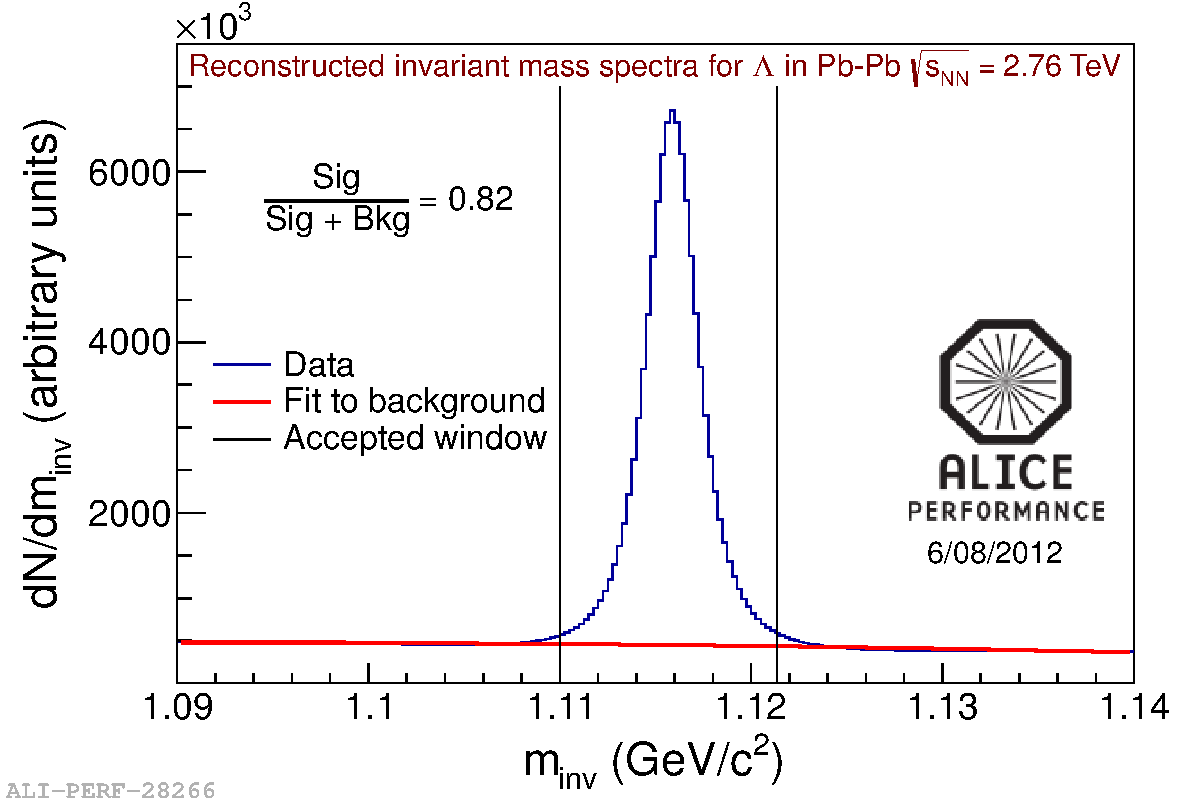
\includegraphics[scale=0.6]{2012-Aug-07-LamInvMass_Perf.pdf}
\caption[Invariant mass distribution for reconstructed $\Lambda$]{Invariant mass distribution for reconstructed $\Lambda$ using the main analysis cuts.  The red line shows a fourth order polynomial fit to the background, which is used to estimate the number of real and accidental $\Lambda$.  The estimated ratio of real $\Lambda$ to all reconstructed $\Lambda$ in the signal region ($ 1.11 < m_{\rm inv} < 1.12136$ GeV/${\rm c^2}$) shown in this plot is approximately 0.82.  Candidate for performance status.}
\label{fig:MassLooseCut}
\end{figure}

\begin{figure}[hbtp]
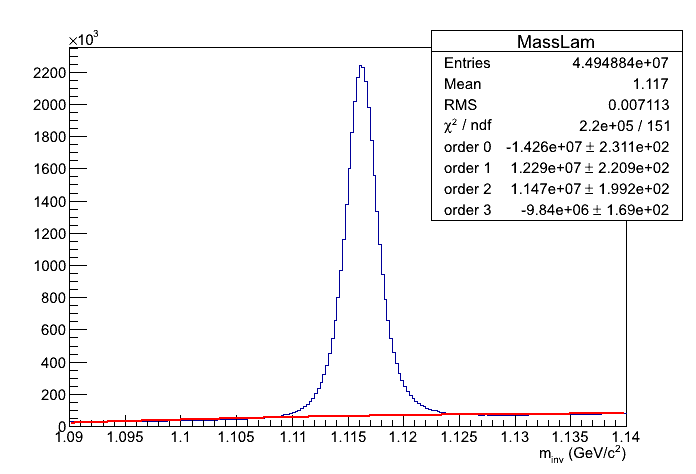
\includegraphics[scale=0.5]{11h_V0_MassLam_TightCuts.png}
\caption[Invariant mass distribution for reconstructed $\Lambda$ using tight cuts]{Invariant mass distribution for reconstructed $\Lambda$ using tight cuts.  Here, $sig/(sig+bkg) \approx 0.92$.}
\label{fig:MassTightCut}
\end{figure}
		


\begin{figure}[hbtp]
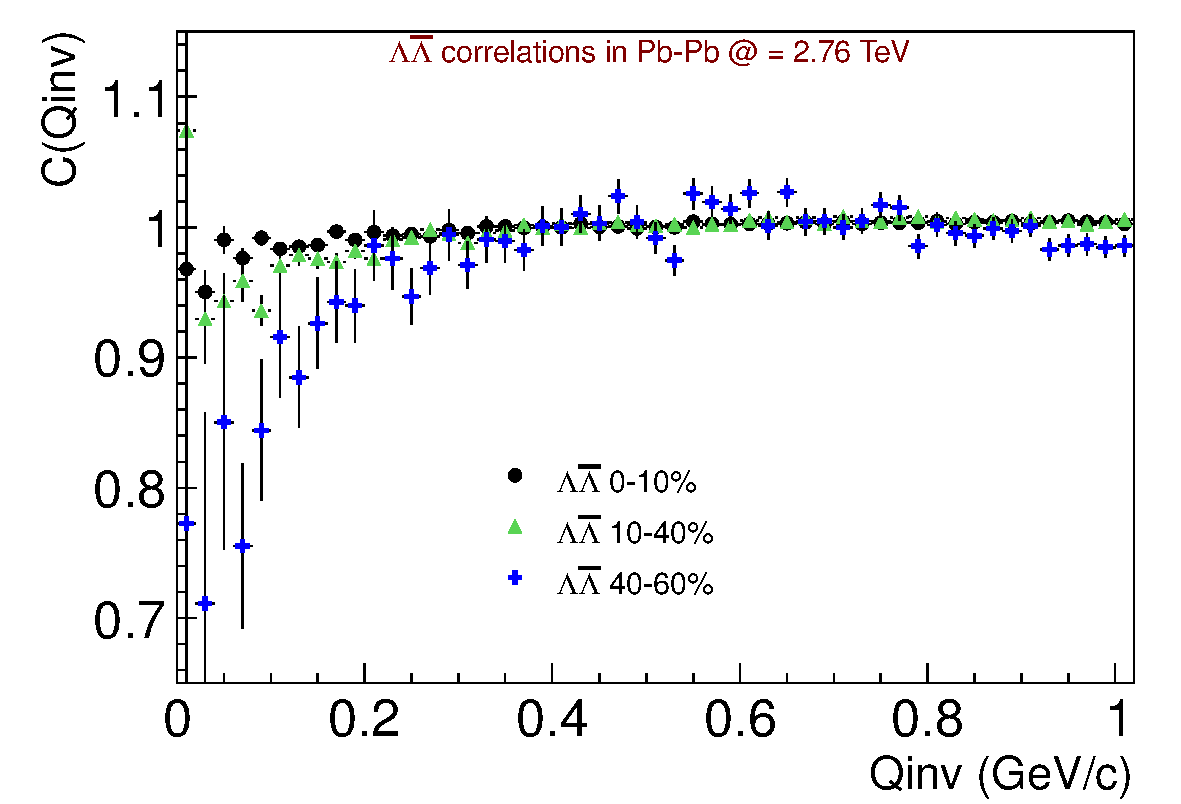
\includegraphics[scale=0.7]{LamALamCF_LooseCuts.pdf}
\caption[Correlation functions versus $q_{\rm inv}$ for $\Lambda\bar{\Lambda}$ pairs in three centrality ranges.]{Correlation functions versus $q_{\rm inv}$ for $\Lambda\bar{\Lambda}$ pairs.  Results are shown for the 0-10\%, 10-40\%, and 40-60\% centrality range.}
\label{fig:CFMixCentralities}
\end{figure}

\begin{figure}[hbtp]
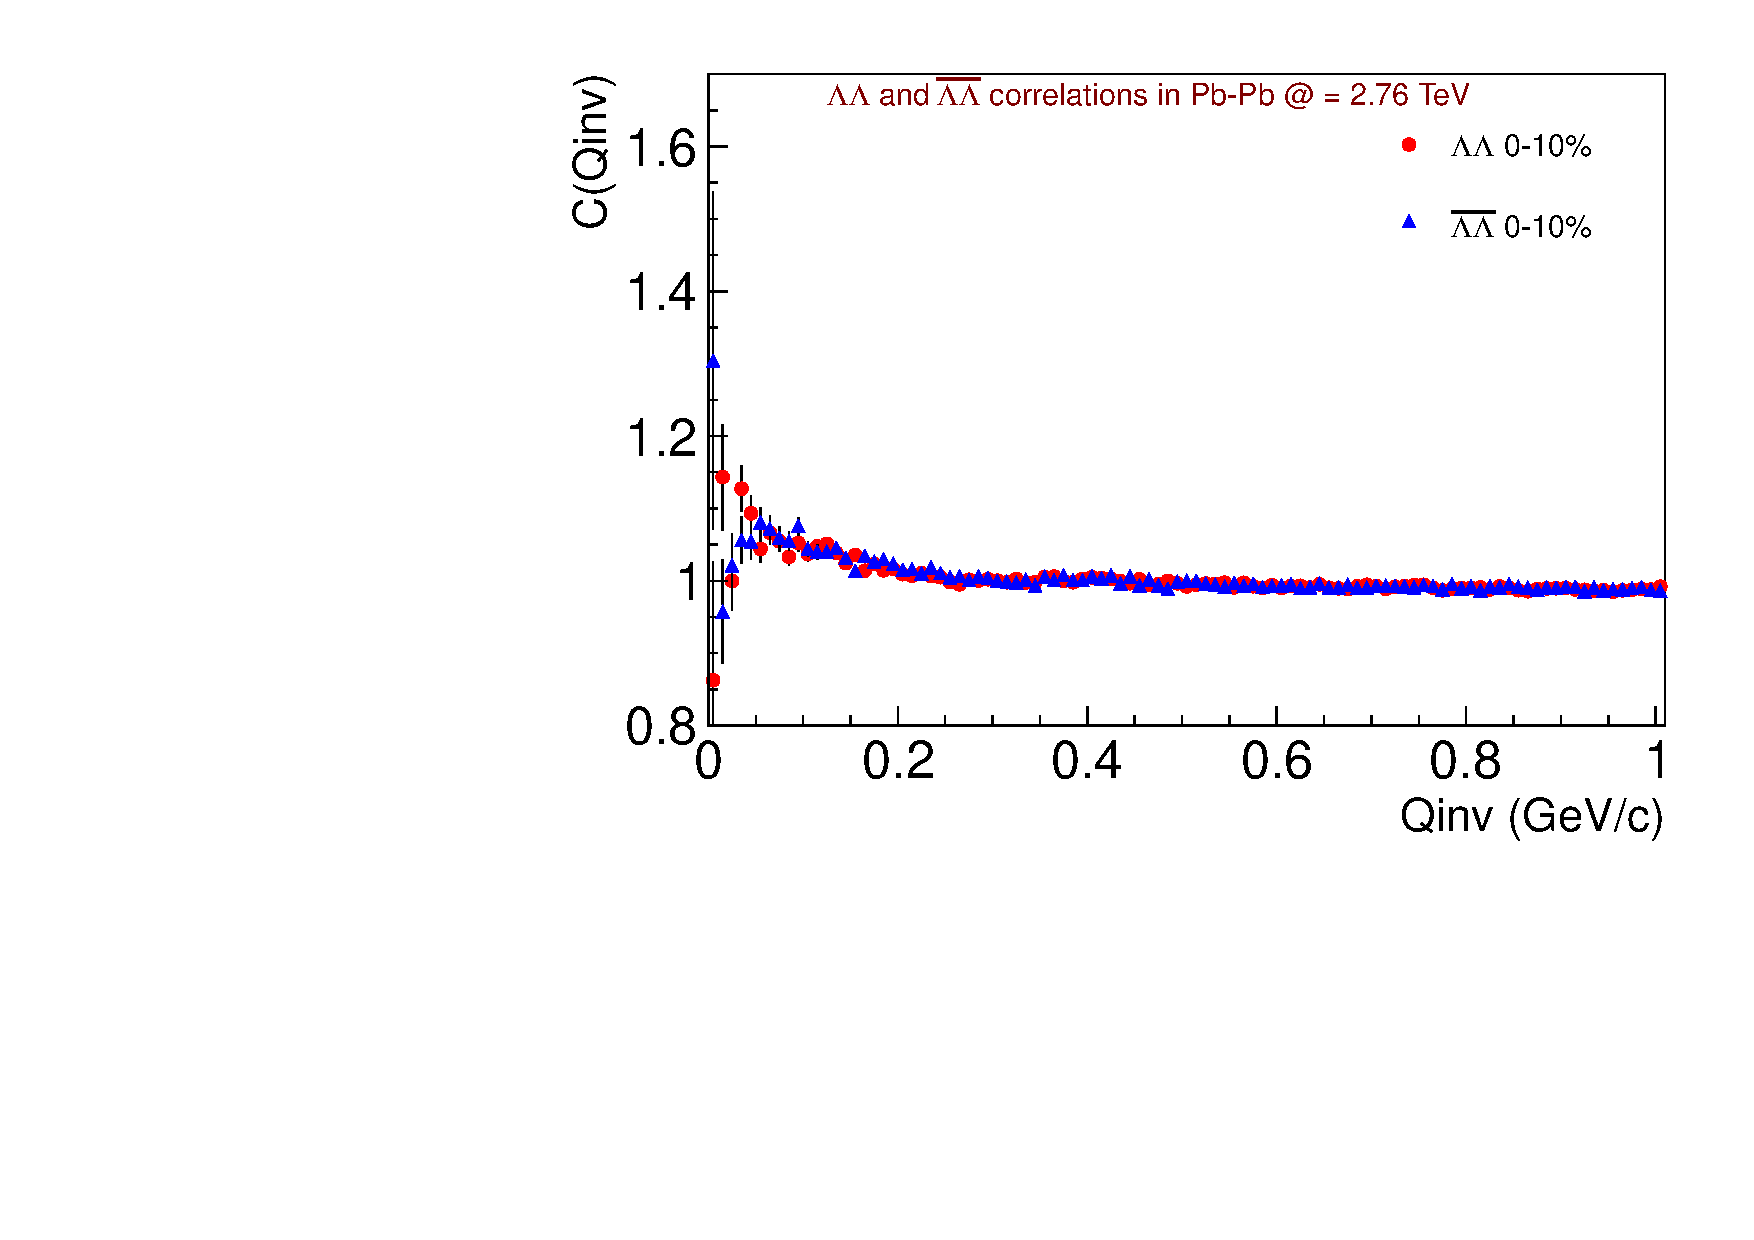
\includegraphics[scale=0.7]{CFs_main_note.pdf}
\caption[Correlation functions versus $q_{\rm inv}$ for $\Lambda\Lambda$ and $\bar{\Lambda}\bar{\Lambda}$ pairs.]{Correlation functions versus $q_{\rm inv}$ for $\Lambda\Lambda$ and $\bar{\Lambda}\bar{\Lambda}$ pairs.  Results are shown for the 0-10\% centrality range.}
\label{fig:CF}
\end{figure}

\begin{figure}[hbtp]
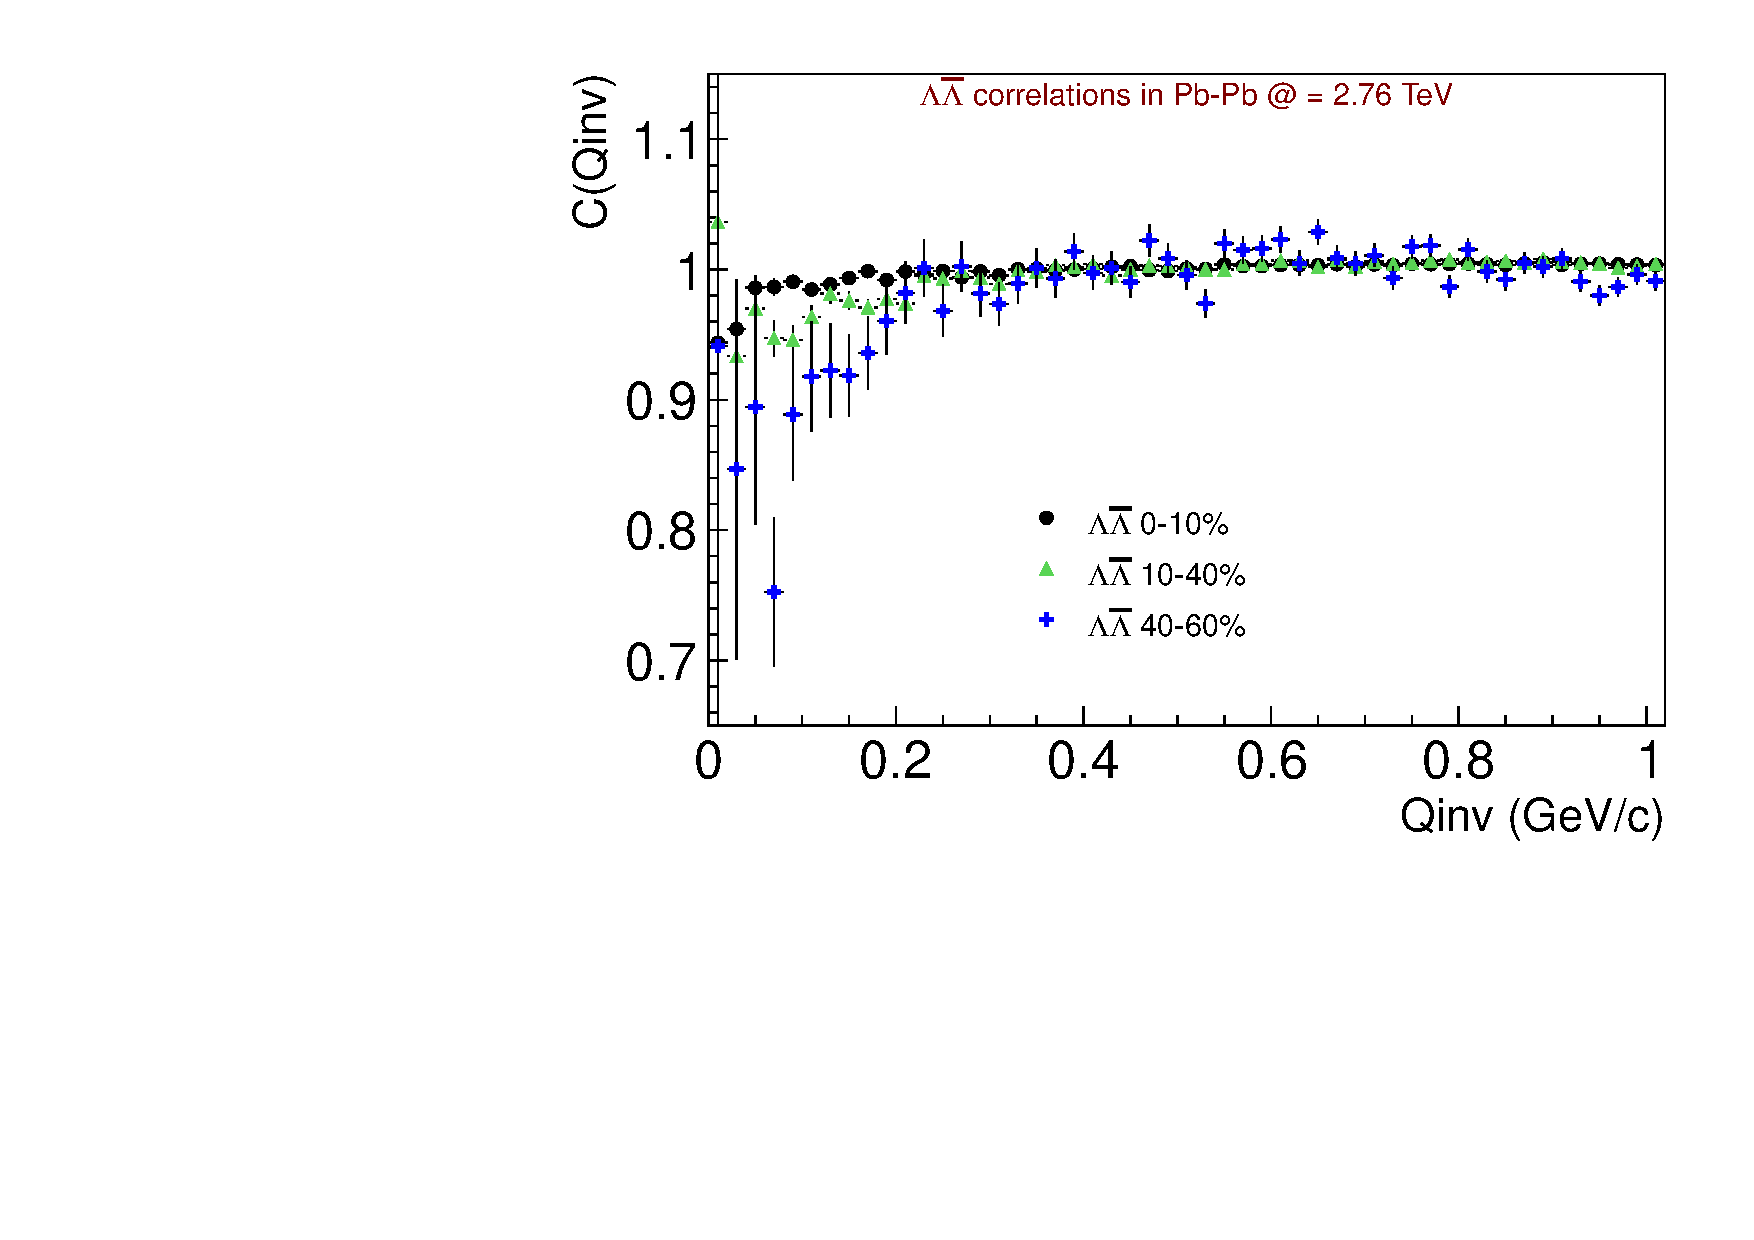
\includegraphics[scale=0.7]{MixCFs_No_MergeCut.pdf}
\caption[Correlation functions versus $q_{\rm inv}$ for $\Lambda\bar{\Lambda}$ pairs in three centrality ranges. No merging cuts]{Correlation functions versus $q_{\rm inv}$ for $\Lambda\bar{\Lambda}$ pairs (without cut on the average separation distance of the daughter pairs).  Results are shown for the 0-10\%, 10-40\%, and 40-60\% centrality range.}
\label{fig:CFNoMergeMix}
\end{figure}

\begin{figure}[hbtp]
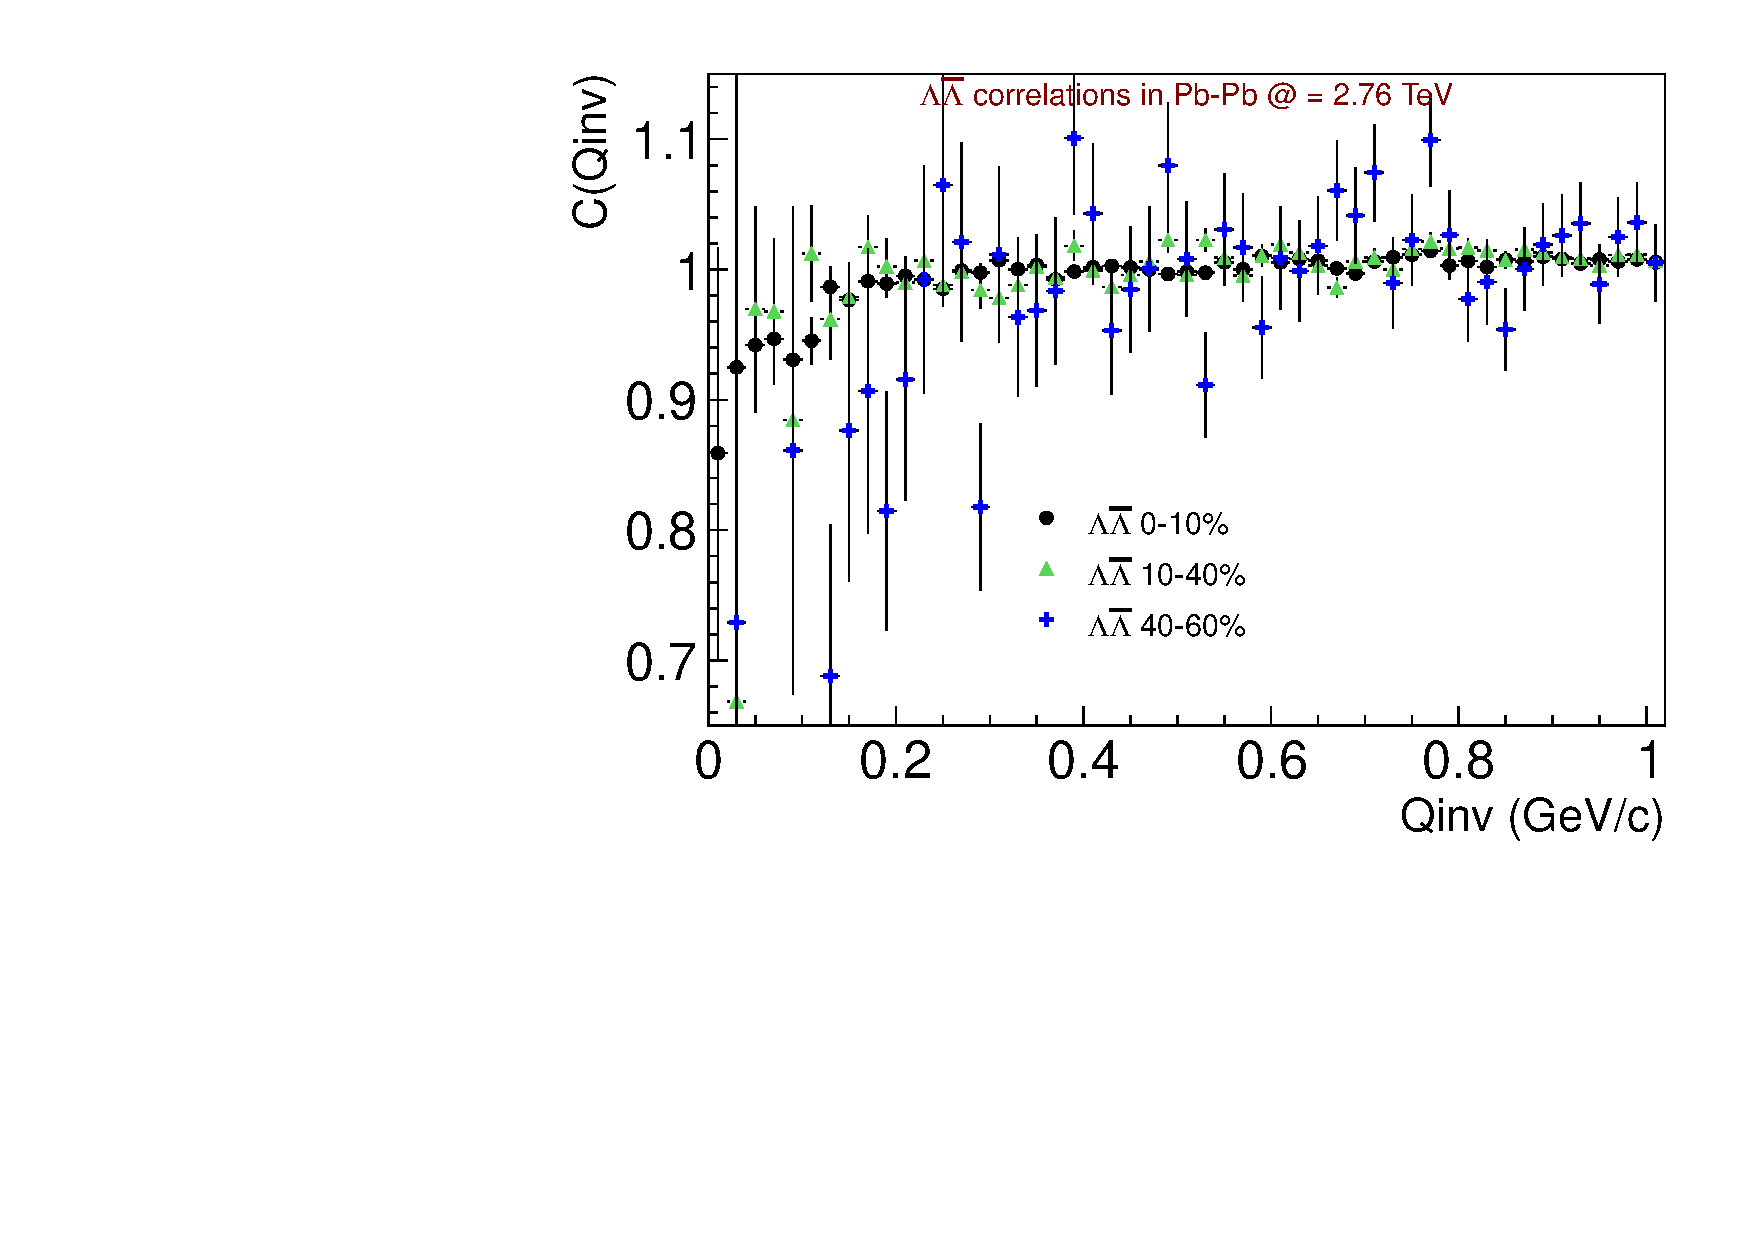
\includegraphics[scale=0.7]{Mix_Tight_cuts_ANote.pdf}
\caption{Correlation functions versus $q_{\rm inv}$ for $\Lambda\bar{\Lambda}$ pairs in three centrality ranges. Tight cuts.}
\label{fig:CFTightCutsMix}
\end{figure}

\begin{figure}[hbtp]
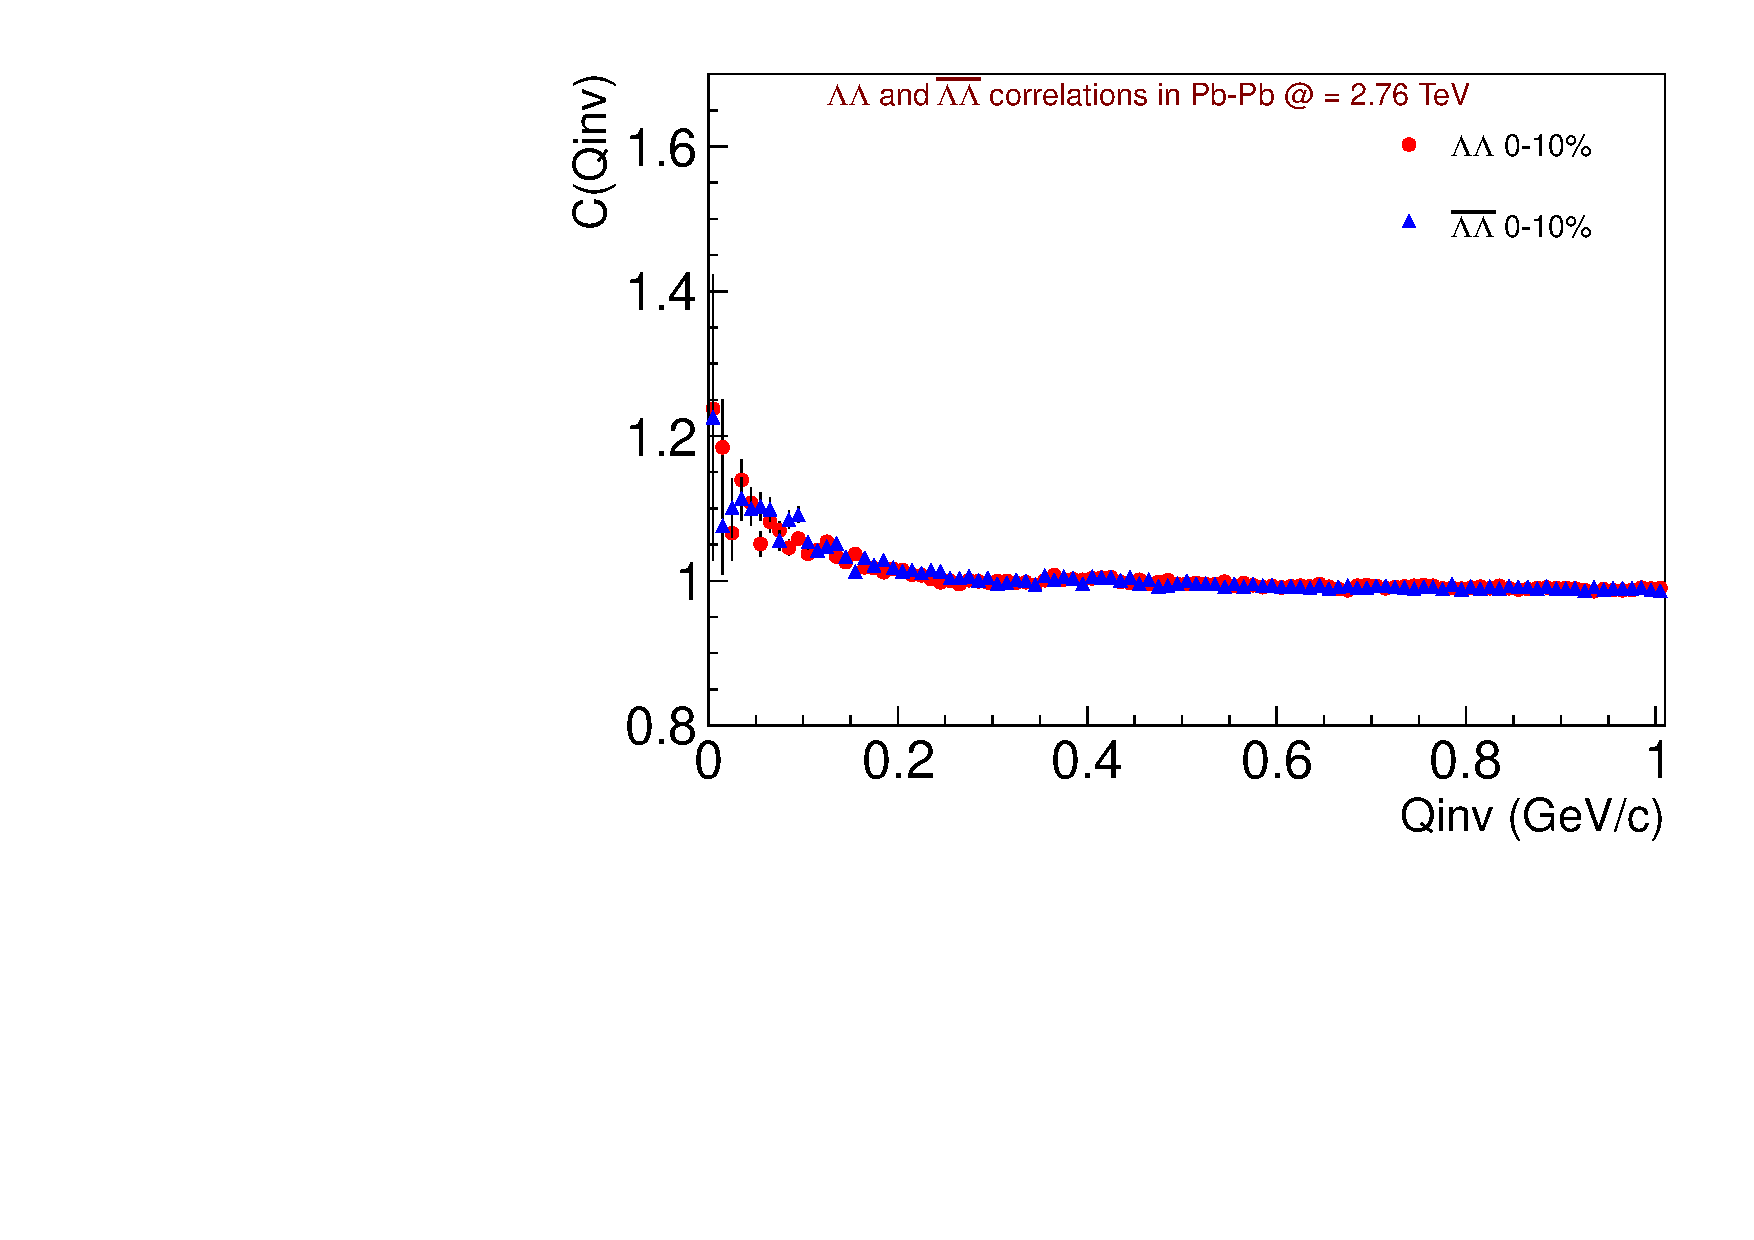
\includegraphics[scale=0.7]{CFs_noMergeCut_note.pdf}
\caption[Correlation functions versus $q_{\rm inv}$ for $\Lambda\Lambda$ and $\bar{\Lambda}\bar{\Lambda}$ pairs. No merging cuts]{Correlation functions versus $q_{\rm inv}$ for $\Lambda\Lambda$ and $\bar{\Lambda}\bar{\Lambda}$ pairs (without cut on the average separation distance of the daughter pairs).  Results are shown for the 0-10\% centrality range.}
\label{fig:CFNoMerge}
\end{figure}

\begin{figure}[hbtp]
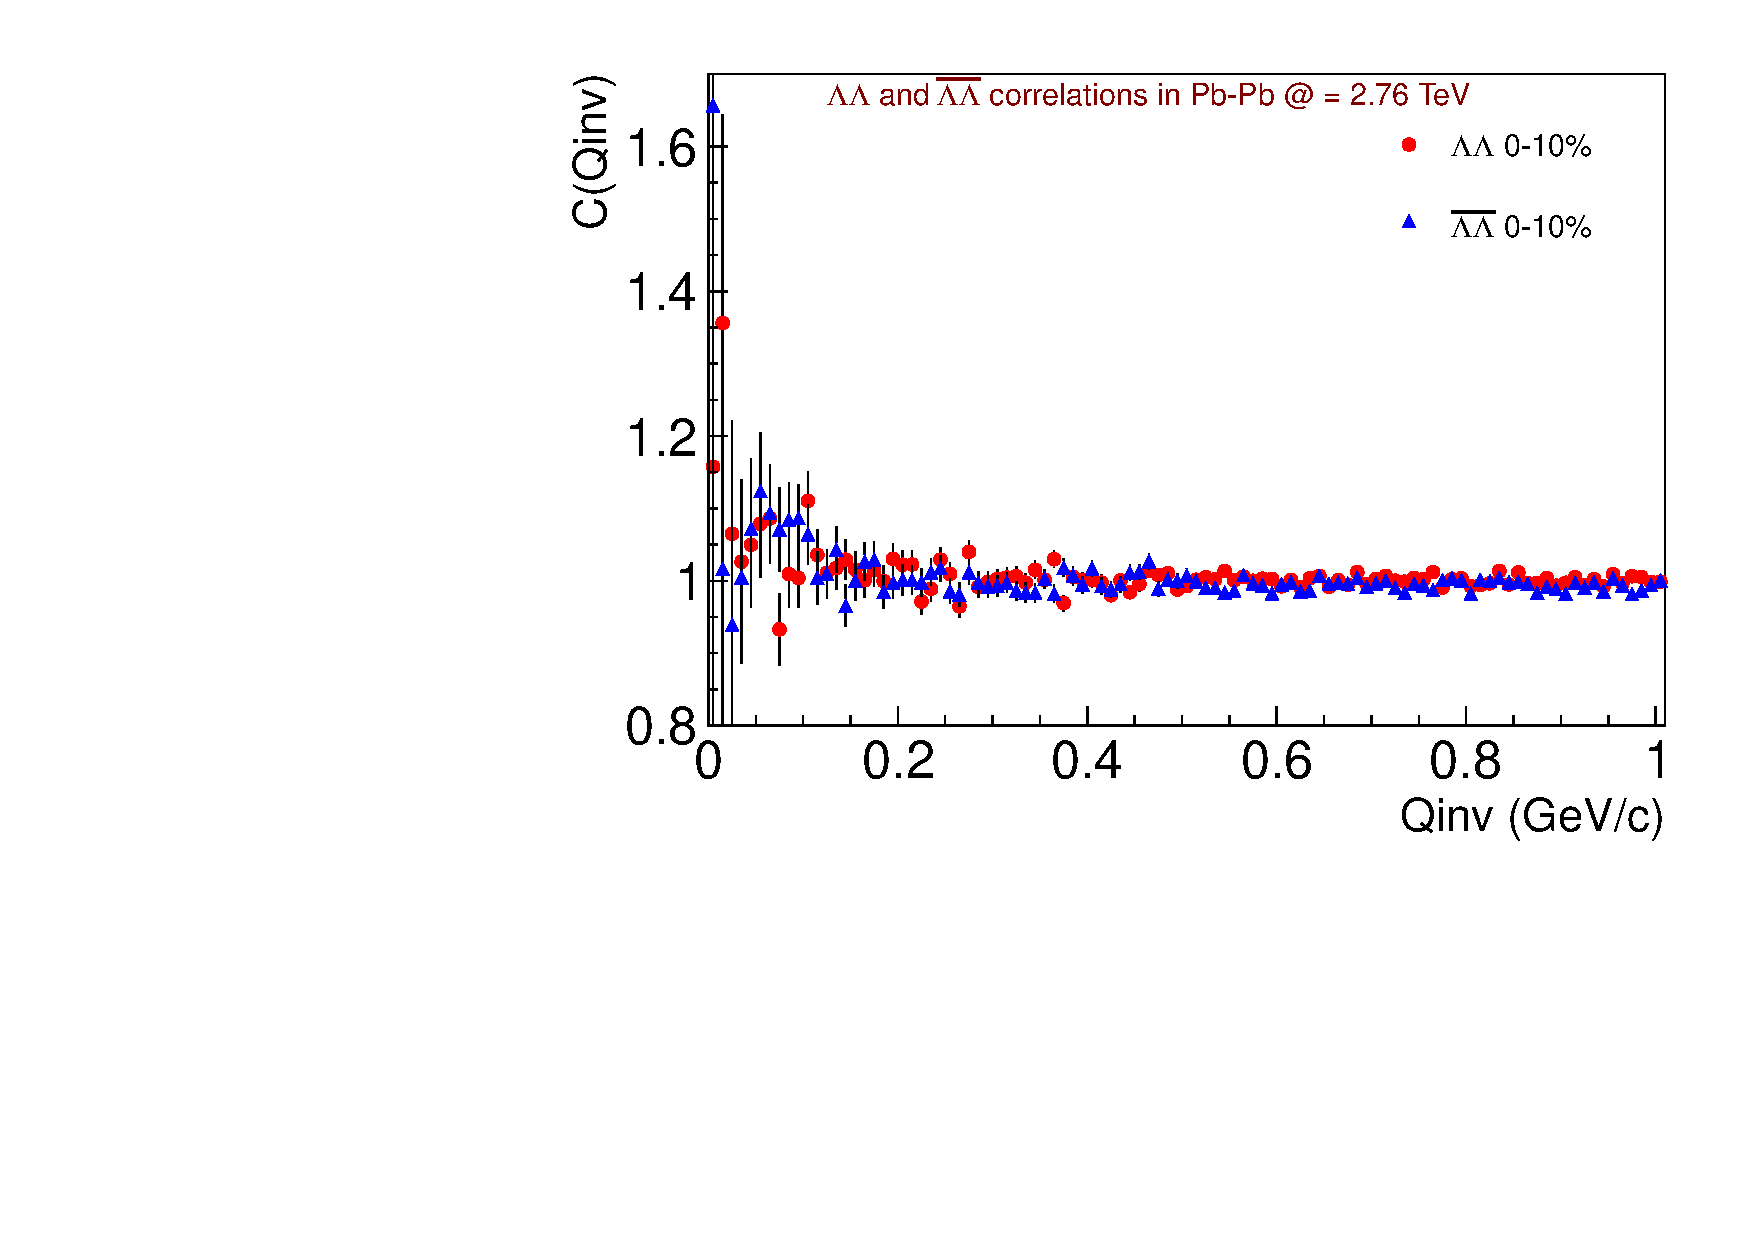
\includegraphics[scale=0.7]{CFs_tightcut_note.pdf}
\caption[Correlation functions versus $q_{\rm inv}$ for $\Lambda\Lambda$ and $\bar{\Lambda}\bar{\Lambda}$ pairs.  Tight cuts]{Correlation functions versus $q_{\rm inv}$ for $\Lambda\Lambda$ and $\bar{\Lambda}\bar{\Lambda}$ pairs using tight reconstruction cuts.  Results are shown for the 0-10\% centrality range.}
\label{fig:CFTightCuts}
\end{figure}

\begin{figure}[hbtp]
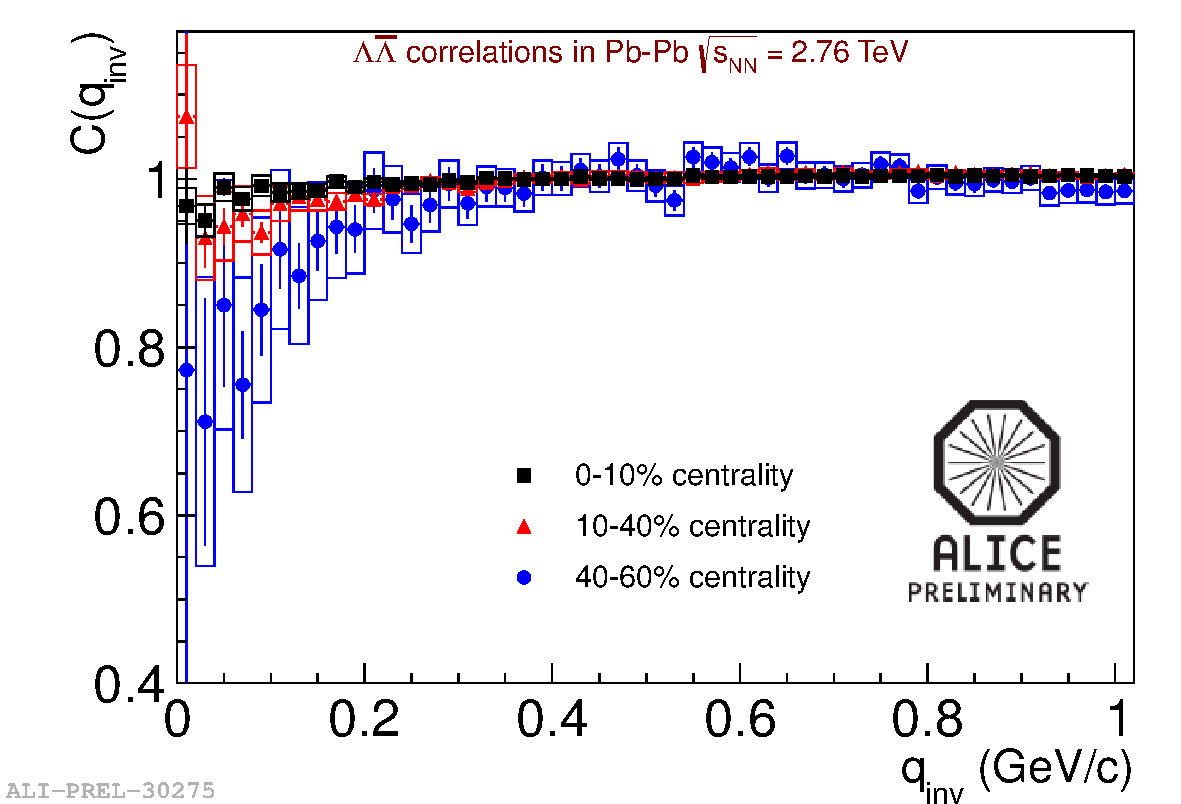
\includegraphics[scale=0.7]{2012-Jul-25-LamALamPrelim.pdf}
\caption[Correlation functions versus $q_{\rm inv}$ for $\Lambda\bar{\Lambda}$ pairs in three centrality ranges with systematic errors.]{Correlation functions versus $q_{\rm inv}$ with systematic errors for $\Lambda\bar{\Lambda}$ pairs. Systematics are computed by fitting the absolute value of the difference between Figure \ref{fig:CFMixCentralities} and Figure \ref{fig:CFTightCutsMix} with a 5th order polynormial. Results are shown for the 0-10\%, 10-40\%, and 40-60\% centrality range.}
\label{fig:CFMixSystematics}
\end{figure}

\bibliographystyle{plain}
\bibliography{bibfile}





%\end{document}